Diktat does AST-analysis, using Abstract Syntax Tree for creation of internal representation (IR) from the parsed code by the kotlin-compiler. This chapter describes how diktat works.

\subsection{ktlint}
To quickly and efficiently analyze the program code, you first need to transform it into a convenient data structure. This is exactly what ktlint does - it parses plain text code into an abstract syntax tree. So we decided not to choose the way of development that was chosen by Facebook in ktfmt and not invent our own framework for parsing the code. We decided to write our own Ruleset on the top of ktlint framework. The good thing is that we were able to inject our set of rules to ktlint via Java's \texttt{ServiceLoader}\footnote{\url{https://docs.oracle.com/javase/8/docs/api/java/util/ServiceLoader.html}}

 In ktlint, the transformation of code happens in the \textsl{prepareCodeForLinting}\footnote{\url{https://github.com/pinterest/ktlint/blob/master/ktlint-core/src/main/kotlin/com/pinterest/ktlint/core/KtLint.kt}} method. This method uses kotlin-compiler-embeddable library to create a root node of type FILE.
For example, this simple code:
\begin{lstlisting}[caption={Simple function that will be transformed to AST}, label={lst:example1}, language=Kotlin]
	fun main() {
		println("Hello World")
	}
\end{lstlisting}

will be converted into the following AST:

\tikzstyle{every node}=[draw=black,thick,anchor=west, scale = 0.6]

\begin{tikzpicture}[%
  grow via three points={one child at (0.3,-0.8) and
  two children at (0.3,-0.8) and (0.3,-1.5)},
  scale=0.6,
  edge from parent path={(\tikzparentnode.south) |- (\tikzchildnode.west)}]

  \node {FILE}
    child { node {PACKAGE\underline{ }DIRECTIVE}}
    child { node {IMPORT\underline{ }LIST}}
    child { node {FUN}
        child {node {fun}}
        child {node {WHITE\underline{ }SPACE}}
        child {node {IDENTIFIER}}
        child {node {VALUE\underline{ }PARAMETER\underline{ }LIST}
            child {node {LPAR}}
            child {node {RPAR}}
        }
        child [missing] {}
        child [missing] {}
        child {node {WHITE\underline{ }SPACE}}
        child {node {BLOCK}
            child {node {LBRACE}}
            child {node {WHITE\underline{ }SPACE}}
            child {node {CALL\underline{ }EXPRESSION}
                child {node {REFERENCE\underline{ }EXPRESSION}
                    child {node {IDENTIFIER}}
                }
                child [missing] {}
                child {node {VALUE\underline{ }ARGUMENT\underline{}LIST}
                    child {node {LPAR}}
                    child {node {VALUE\underline{ }ARGUMENT}
                        child {node {STRING\underline{ }TEMPLATE}
                            child {node {OPEN\underline{ }QUOTE}}
                            child {node {LITERAL\underline{ }STRING\underline{ }TEMPLATE\underline{ }ENTRY}
                                child {node {REGULAR\underline{ }STRING\underline{ }PART}}
                            }
                            child [missing] {}
                            child {node {CLOSING\underline{ }QUOTE}}
                        }
                    }
                    child [missing] {}
                    child [missing] {}
                    child [missing] {}
                    child [missing] {}
                    child [missing] {}
                    child [missing] {}
                    child {node {RPAR}}
                }
            }
            child [missing] {}
            child [missing] {}
            child [missing] {}
            child [missing] {}
            child [missing] {}
            child [missing] {}
            child [missing] {}
            child [missing] {}
            child [missing] {}
            child [missing] {}
            child [missing] {}
            child [missing] {}
            child [missing] {}
            child {node {WHITE\underline{ }SPACE}}
            child {node {RBRACE}}
        }
    };
\end{tikzpicture}
\\

If there are error elements inside the constructed tree, then the corresponding error is displayed. If the code is valid and parsed without errors, for each rule in the Ruleset, the \textsl{visit} method is called for the root node itself and its “children” are sequentially passed.
When you run program, you can pass flags to ktlint - one of them is \texttt{-F}. This flag means that the rule will not only report an error, but will also try to fix it.

\subsection{DiKTat}

Another feature of ktlint is that at it's startup you can provide a JAR file with additional ruleset(s), that will be discovered by the \texttt{ServiceLoader} and then all AST nodes will be passed to these rules. DiKTat uses this approach.

The only modification Diktat makes to the framework is that it adds a mechanism to disable Inspection from the code using annotations or configuration file. The set of all rules is described in the \textsl{DiktatRuleSetProvider}\footnote{\url{https://github.com/cqfn/diKTat/blob/v0.1.3/diktat-rules/src/main/kotlin/org/cqfn/diktat/ruleset/rules/DiktatRuleSetProvider.kt}} class. This class overrides the \textsl{get()} method of the \textsl{RuleSetProvider}\footnote{\url{https://github.com/pinterest/ktlint/blob/master/ktlint-core/src/main/kotlin/com/pinterest/ktlint/core/RuleSetProvider.kt}} interface, which returns a set of rules to be "traversed". But before returning this set Diktat is reading the configuration file where the user has independently configured all the Inspections. If there is no configuration file, then a warning will be displayed and Inspections will use the default configuration file.
Each rule must implement the \textsl{visit} method of the abstract Rule class, which describes the logic of the rule. By the way it is a special case of a famous pattern Visitor \cite{ref:gang}. Implementation example of the simple Rule that contains one Inspections can be found below.

\begin{lstlisting}[caption={Example of the Rule.}, label={lst:example1}, language=Kotlin]
class SingleLineStatementsRule(private val configRules: List<RulesConfig>) : Rule("statement") {
    private var isFixMode: Boolean = false
    private lateinit var emitWarn: EmitType

    override fun visit(node: ASTNode,
                       autoCorrect: Boolean,
                       emit: EmitType) {
        emitWarn = emit
        isFixMode = autoCorrect

        // all the work is done with ASTNode - this is the type, provided by Kotlin compiler
        node.getChildren(TokenSet.create(SEMICOLON)).forEach {
            if (!it.isFollowedByNewline()) {
                // configuration is checked by warning mechanism under the hood
                // warnings are mapped to proper paragraph of a code standard
                MORE_THAN_ONE_STATEMENT_PER_LINE.warnAndFix(
                        configRules,
                        emitWarn,
                        isFixMode,
                        it.extractLineOfText(),
                        it.startOffset,
                        it
                // this lambda provides the logic that will be used to fix the code
                ) {
                    if (it.treeParent.elementType == ENUM_ENTRY) {
                        node.treeParent.addChild(PsiWhiteSpaceImpl("\n"), node.treeNext)
                    } else {
                        if (!it.isBeginByNewline()) {
                            val nextNode = it.parent(
                                    { parent -> parent.treeNext != null },
                                    strict = false
                            )?.treeNext

                            node.appendNewlineMergingWhiteSpace(nextNode, it)
                        }
                        node.removeChild(it)
                    }
                }
            }
        }
    }
}
\end{lstlisting}

The example above describes the Rule that checks that there are no statements separated by a semicolon. The list of configurations is passed to the parameter of this rule so that the error is displayed only when the Rule is enabled (further it will be described how to enable or disable the Rule). The class fields and the \textsl{visit()} method are described below. The first parameter in method is of \textsl{ASTNode} type, this type is produced by the Kotlin compiler. It is important to understand that these visitors are called for each and every node of AST that is provided by the compiler. This is not optimal from the perspective of the performance, but makes the code much more readable and isolated.

Then a check occurs: if the code contains a line in which more than one statement per line and this rule is enabled, then the rule will be executed and, depending on the mode in which the user started ktlint, the rule will either simply report an error or fix it. In our case, when an error is found, the method is called to report and fix the error - \textsl{warnAndFix()}.

All warnings that contain similar logic (e.g. regarding formatting of function KDocs) are checked in the same Rule. This way we can make small optimisation and check similar parts of AST only once. Whether the Inspection is enabled or disabled is checked inside \textsl{warn()} or \textsl{warnAndFix()} methods. The same works for the suppression of Inspections: right before emitting the warning we check whether any of current node's parents has a Suppress annotation. The diagram below describes it's architecture:

\begin{figure}[H]
    \centering
    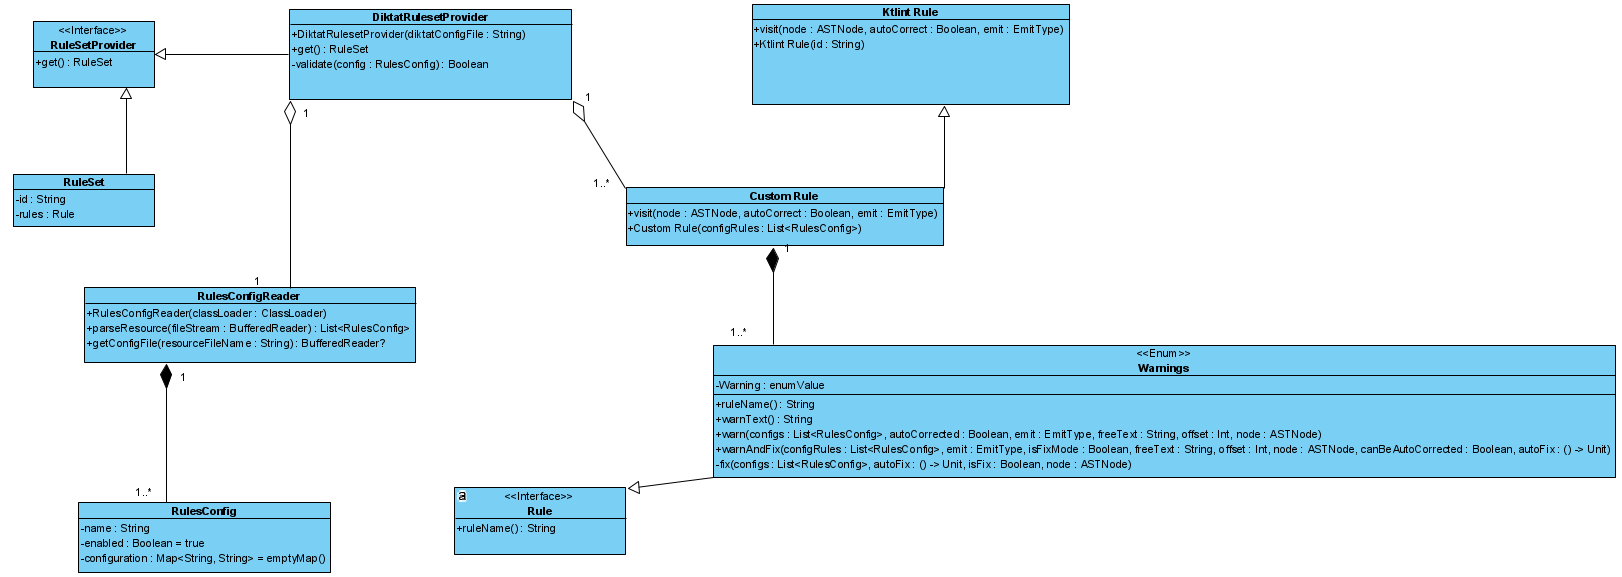
\includegraphics[scale=0.5]{pictures/class.PNG}
    \caption{Diktat class diagram}
    \label{fig:top_languages}
\end{figure}


\subsection{Examples of unique inspections}
\par
As already described above, DiKTat has more rules than existing analogues, therefore, it will find and fix more errors and shortcomings and, thereby, make the code cleaner and better. To better understand how detailed are checks in Diktat,let's mention a few examples:

\begin{enumerate}
    \item \textbf{Package.}
In DiKTat, there are about 6 Inspections that are checking the package naming. For comparison: detekt has only one rule, where the package name is simply checked by a pattern, in ktlint there are zero inspections.
    \item \textbf{KDoc.}
KDoc is an important part of good code to make it easier to understand and navigate the program. In DiKTat there are 15 rules on KDoc, in detekt there are only 7. Therefore, DiKTat will make and correct KDoc in more detail and correctly.
\end{enumerate}

There are also many unique Inspections that other analyzers do not have. Here are some of them:

\begin{enumerate}
    \item \textbf{COMMENTED\underline{ }OUT\underline{ }CODE} – This Inspection checks if the code contains commented code blocks.
    \item \textbf{FILE\underline{ }CONTAINS\underline{ }ONLY\underline{ }COMMENTS} – This rule checks file contains not only comments.
    \item \textbf{LOCAL\underline{ }VARIABLE\underline{ }EARLY\underline{ }DECLARATION} – This rule checks that local variables are declared close to the point where they are first used.
    \item \textbf{AVOID\underline{ }NESTED\underline{ }FUNCTIONS} - This rule checks for nested functions and warns and fixes if it finds any. An example of changing the tree when this rule is triggered and DiKTat is run with fix mode:\\\\
    \begin{tikzpicture}[%
  grow via three points={one child at (0.3,-0.8) and
  two children at (0.3,-0.8) and (0.3,-1.5)},
  scale=0.5,
  edge from parent path={(\tikzparentnode.south) |- (\tikzchildnode.west)}]
    
  \node(a) {...}
    child { node {FUN}
        child {node {...}}
        child {node {BLOCK}            
            child {node {FUN}
            	child{node{...}}
		child{node{BLOCK}
			child{node{...}}
		}
            }
        }
    };
    
    \node(b) [right of=a, xshift=17cm]{...}
    	child { node {FUN}
        		child {node {...}}
        		child {node {BLOCK}          
          		child{node{...}}
		}	
        }
        child [missing] {}
	child [missing] {}
         child { node {FUN}
        		child {node {...}}
        		child {node {BLOCK}          
          		child{node{...}}
		}	
        };
     
    \draw[-latex,very thick,shorten <=5mm,shorten >=5mm,] ([xshift=5cm,yshift=-3cm]a.north) to ([xshift=-2cm, yshift=-3cm]b.north);
\end{tikzpicture}
\\
    \item \textbf{FLOAT\underline{ }IN\underline{ }ACCURATE\underline{ }CALCULATIONS} - Inspection that checks that floating-point numbers are not used for accurate calculations (see the corresponding Rule from the code style to get more information).

    \item \textbf{PACKAGE\underline{ }NAMING} - This Inspection checks that package name is in a proper format and is separated by dots. This inspection is very demonstrative to show how the work with AST is done.
    
    This inspection receives different nodes and checks them one by one. First it checks their element type (type of the node in AST). When it's element type equals to \texttt{PACKAGE\_DIRECTIVE} it gets the file name and collects all nodes with \texttt{IDENTIFIER} type as it is shown on the following graph:
    
        
\begin{center}
\begin{tikzpicture}[nodes={draw, circle}, sibling distance=1.5cm, level distance = 1.2cm, minimum size=3.1cm, scale = 1.2, node distance=16cm]
\node(main)[text width = 2cm] { PACKAGE DIRECTIVE}
    child { node(a) [below left] { PACKAGE} }
    child { node(b)[below] { WHITE SPACE} }
    child { node(c)[below right, text width=3cm] {  DOT QUALIFIED EXPRESSION} 
        child { node(d)[below left, text width=2.5cm] { REFERENCE EXPRESSION}
            child { node(e)[below, fill = selectColor] { IDENTIFIER} }
        }
        child { node(f)[below] { DOT} }
        child { node(g)[below right, text width=2.5cm] { REFERENCE EXPRESSION}
            child { node(h)[below, fill = selectColor] { IDENTIFIER} }
        }
    };
    \draw[->, line width = 0.5mm] (main) -- (a);
    \draw[->, line width = 0.5mm] (main) --(b);
    \draw[->, line width = 0.5mm] (main) -- (c);
    \draw[->, line width = 0.5mm] (c) -- (d);
    \draw[->, line width = 0.5mm] (d) -- (e);
    \draw[->, line width = 0.5mm] (c) -- (f);
    \draw[->, line width = 0.5mm] (c) -- (g);
    \draw[->, line width = 0.5mm] (g)  --(h);

\end{tikzpicture}
\end{center}
    
In order to collect  elements with a proper type, Inspection has to do a tree traversal. Tree traversal is done by a special method called \texttt{findAllNodesWithCondition()} (see Listing 3). This function searches for a node with a given condition (in this case it is when node's type equals to \texttt{IDENTIFIER}). As a basis it uses DFS (Depth-first search): it goes recursively in depth of the tree and compares types of AST nodes. When it finds necessary node it returns it and the result from it's parent search as a list, otherwise it returns empty list. At the end the Inspection checks the package name based on identifiers and file name. 


\begin{lstlisting}[caption={Method for AST traversal}, label={lst:example1}, language=Kotlin]      
/**
 * This method performs tree traversal and returns all nodes which satisfy the condition
 */
fun ASTNode.findAllNodesWithCondition(condition: (ASTNode) -> Boolean, withSelf: Boolean = true): List<ASTNode> {
    val result = if (condition(this) && withSelf) mutableListOf(this) else mutableListOf()
    return result + this.getChildren(null).flatMap {
        it.findAllNodesWithCondition(condition)
    }
}
\end{lstlisting}

\tikzstyle{every node}=[draw=black,thick,anchor=west, scale = 0.5, font = \large]
\end{enumerate}